
\chapter{Test d'intégration}

Nous n'avons malheureusement pas pu faire de nombreux tests d'intégrations puisque à la fin de notre projet nous n'avions pas la totalité des composants pour monter notre radiogoniomètre. Néanmoins nous avons pu tester l'intégration du radiogoniomètre au \rpi en plaçant des leds sur les ports GPIO, ainsi que l'intégration de l'application mobile au serveur central.


\section{Raspberry Pi}
La documentation technique lié a notre Raspberry Pi es situé en annexe à la page \pageref{annexe:rpi}
~\\

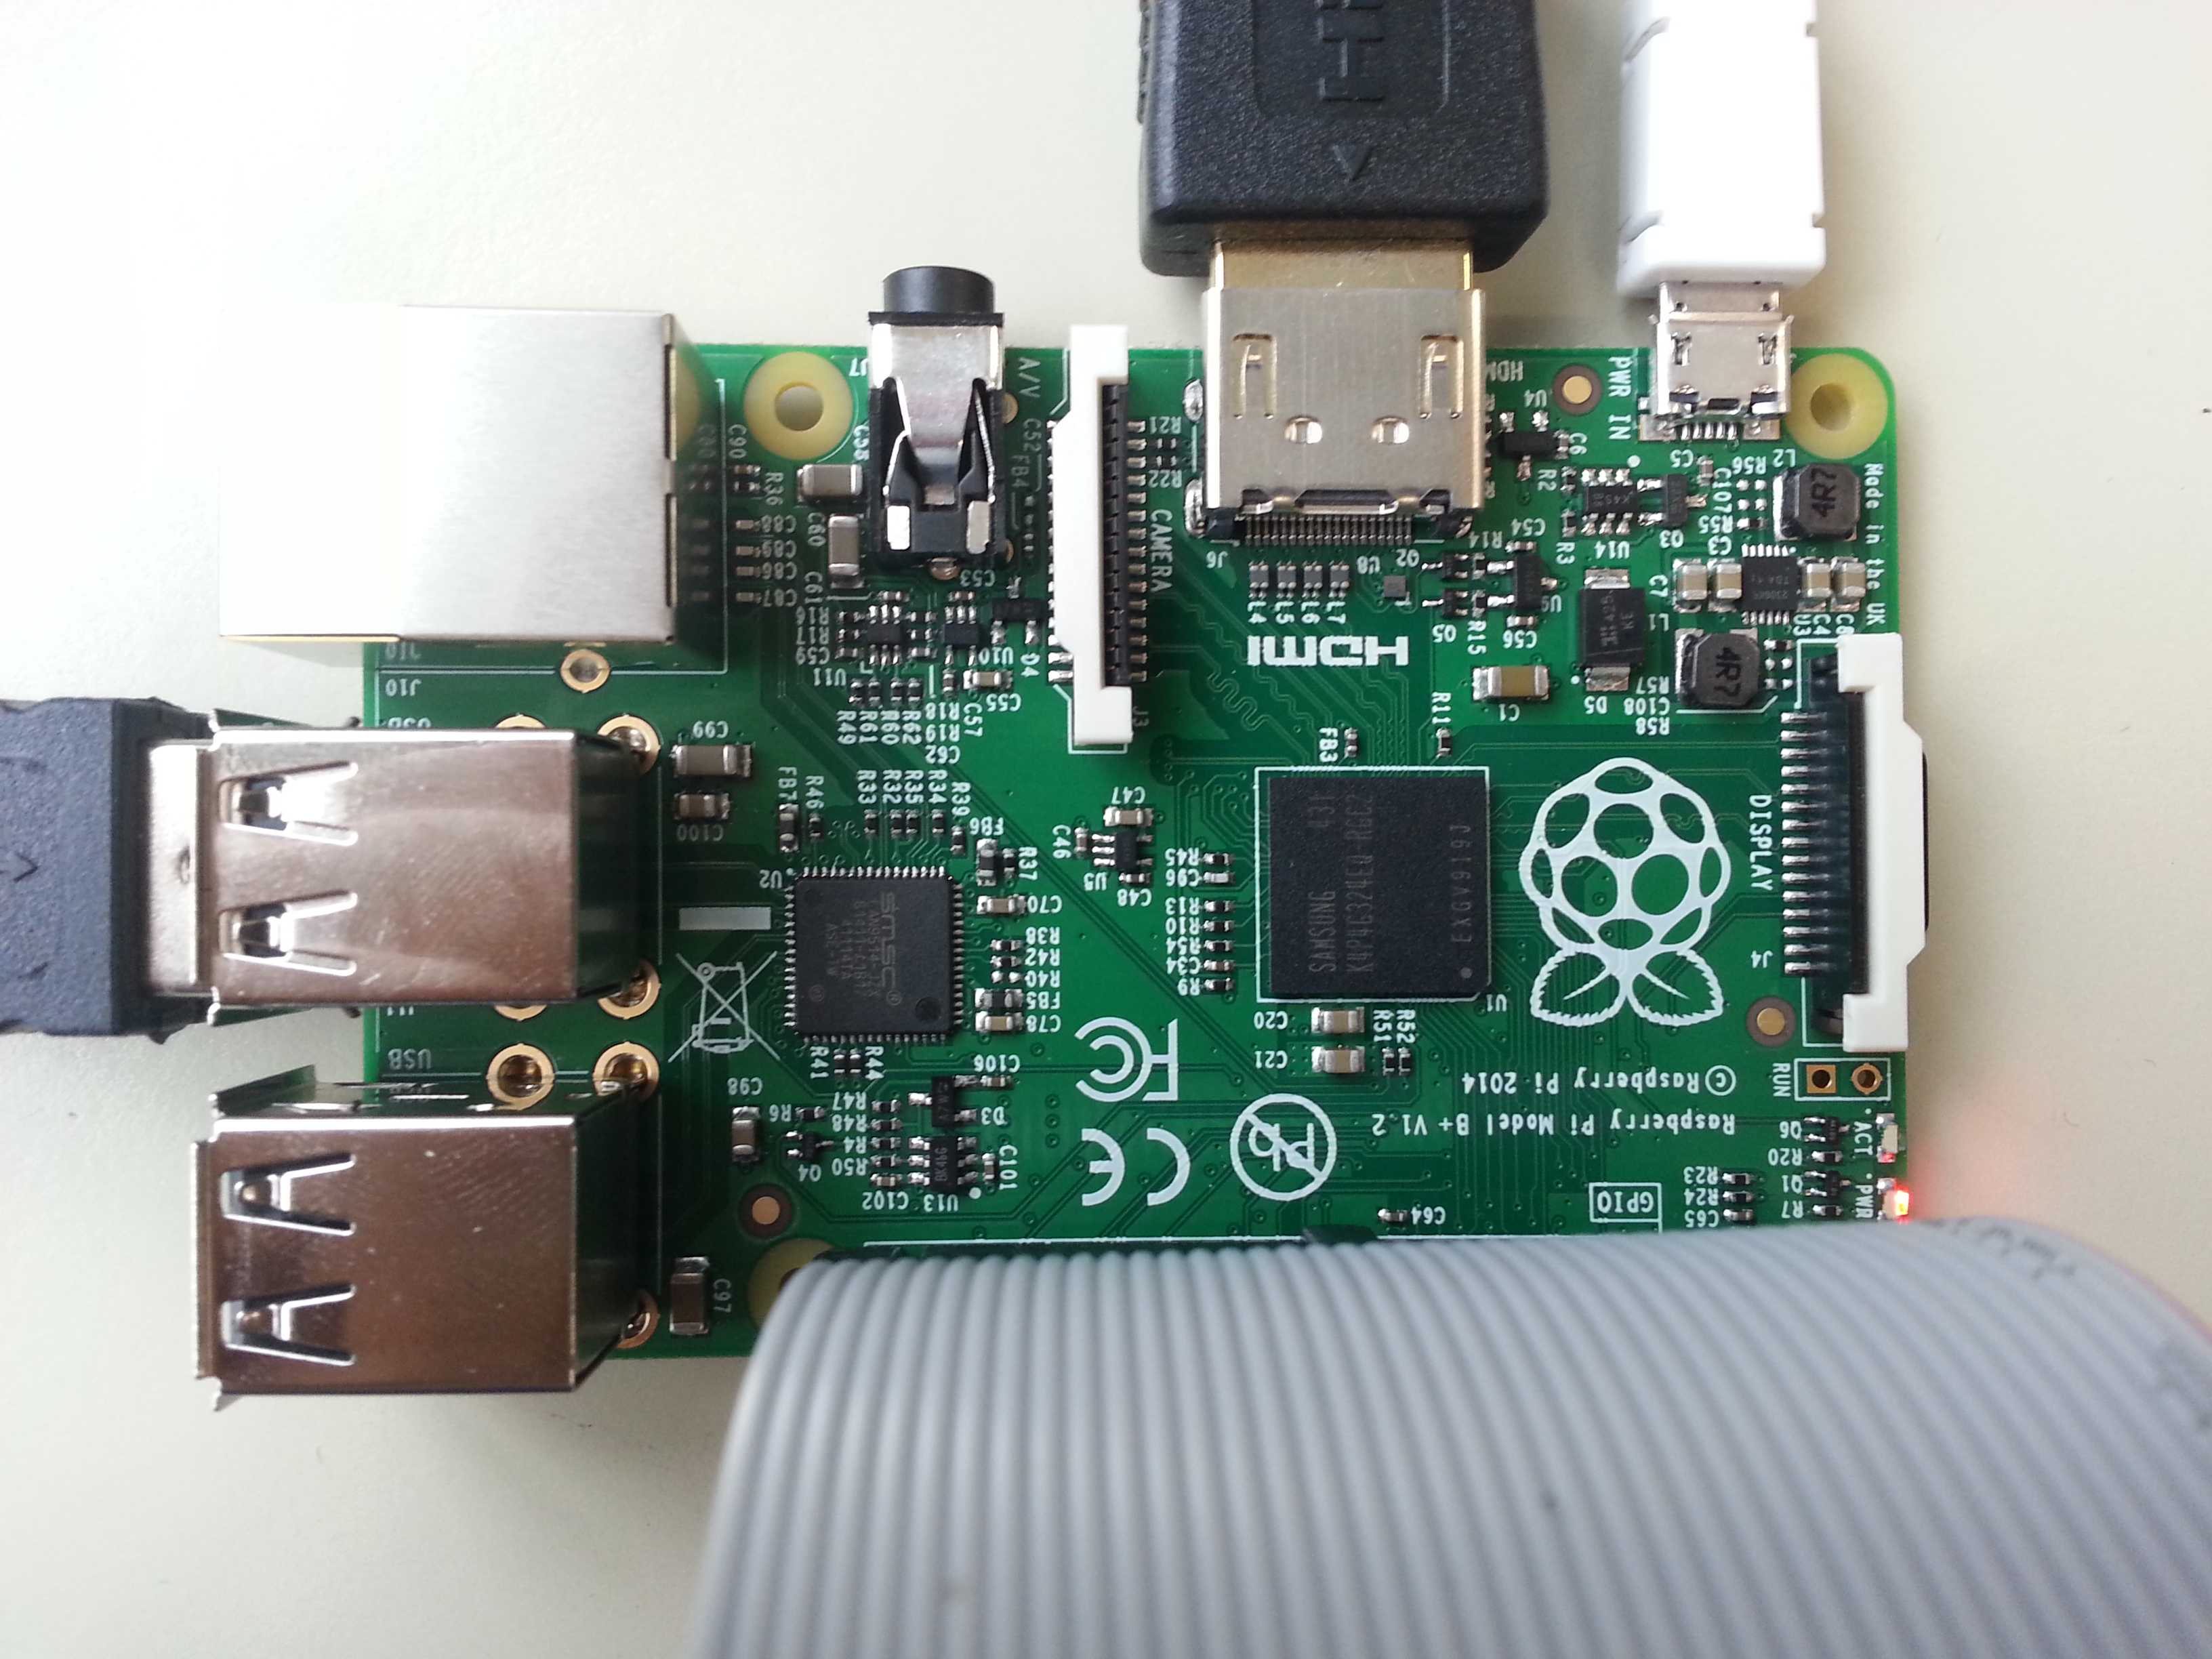
\includegraphics[width=\textwidth]{Test_unitaire/Rpi/img5.jpg}
\captionof{figure}{Notre Raspberry Pi B+}

~\\
\parindent=15pt

Pour s'assurer que notre Raspberry Pi répond aux spécifications fonctionnelles et qu'il fonctionne correctement en toutes circonstances pour notre projet, nous y avons réalisé des tests intégrations.

Après avoir enfin installé le système d'exploitation Raspbian\footnote{La documentation lié à Raspbian est situé en annexe à la page \pageref{annexe:raspbian}} sur notre Raspberry Pi B+, nous avons tenté de tester les ports GPIO. Pour cela, dans un premier temps, nous avons allumé des LED grâce à un script python à travers différents ports GPIO. Sur la figure \ref{figure:led}, on peut observer que nous avons allumé une LED grâce au port 22.
~\\

Dans notre projet le Raspberry Pi sera placé entre le radio-goniomètre à effet Doppler et l'utilisateur. Il aura deux taches, corréler les données entre tous les dispositifs pour obtenir la position du drone et afficher le résultat à l'utilisateur. Pour cela il doit récupérer la direction qui est donné par le Montréal 3v2. Cette position est donnée à travers des LED (voir figure \ref{figure:ledMontreal}). Nous allons donc placer le Raspberry Pi au niveau des LED pour obtenir les informations délivré par le Montréal 3v2. % TODO : A FINIR

\begin{figure}[!h]
  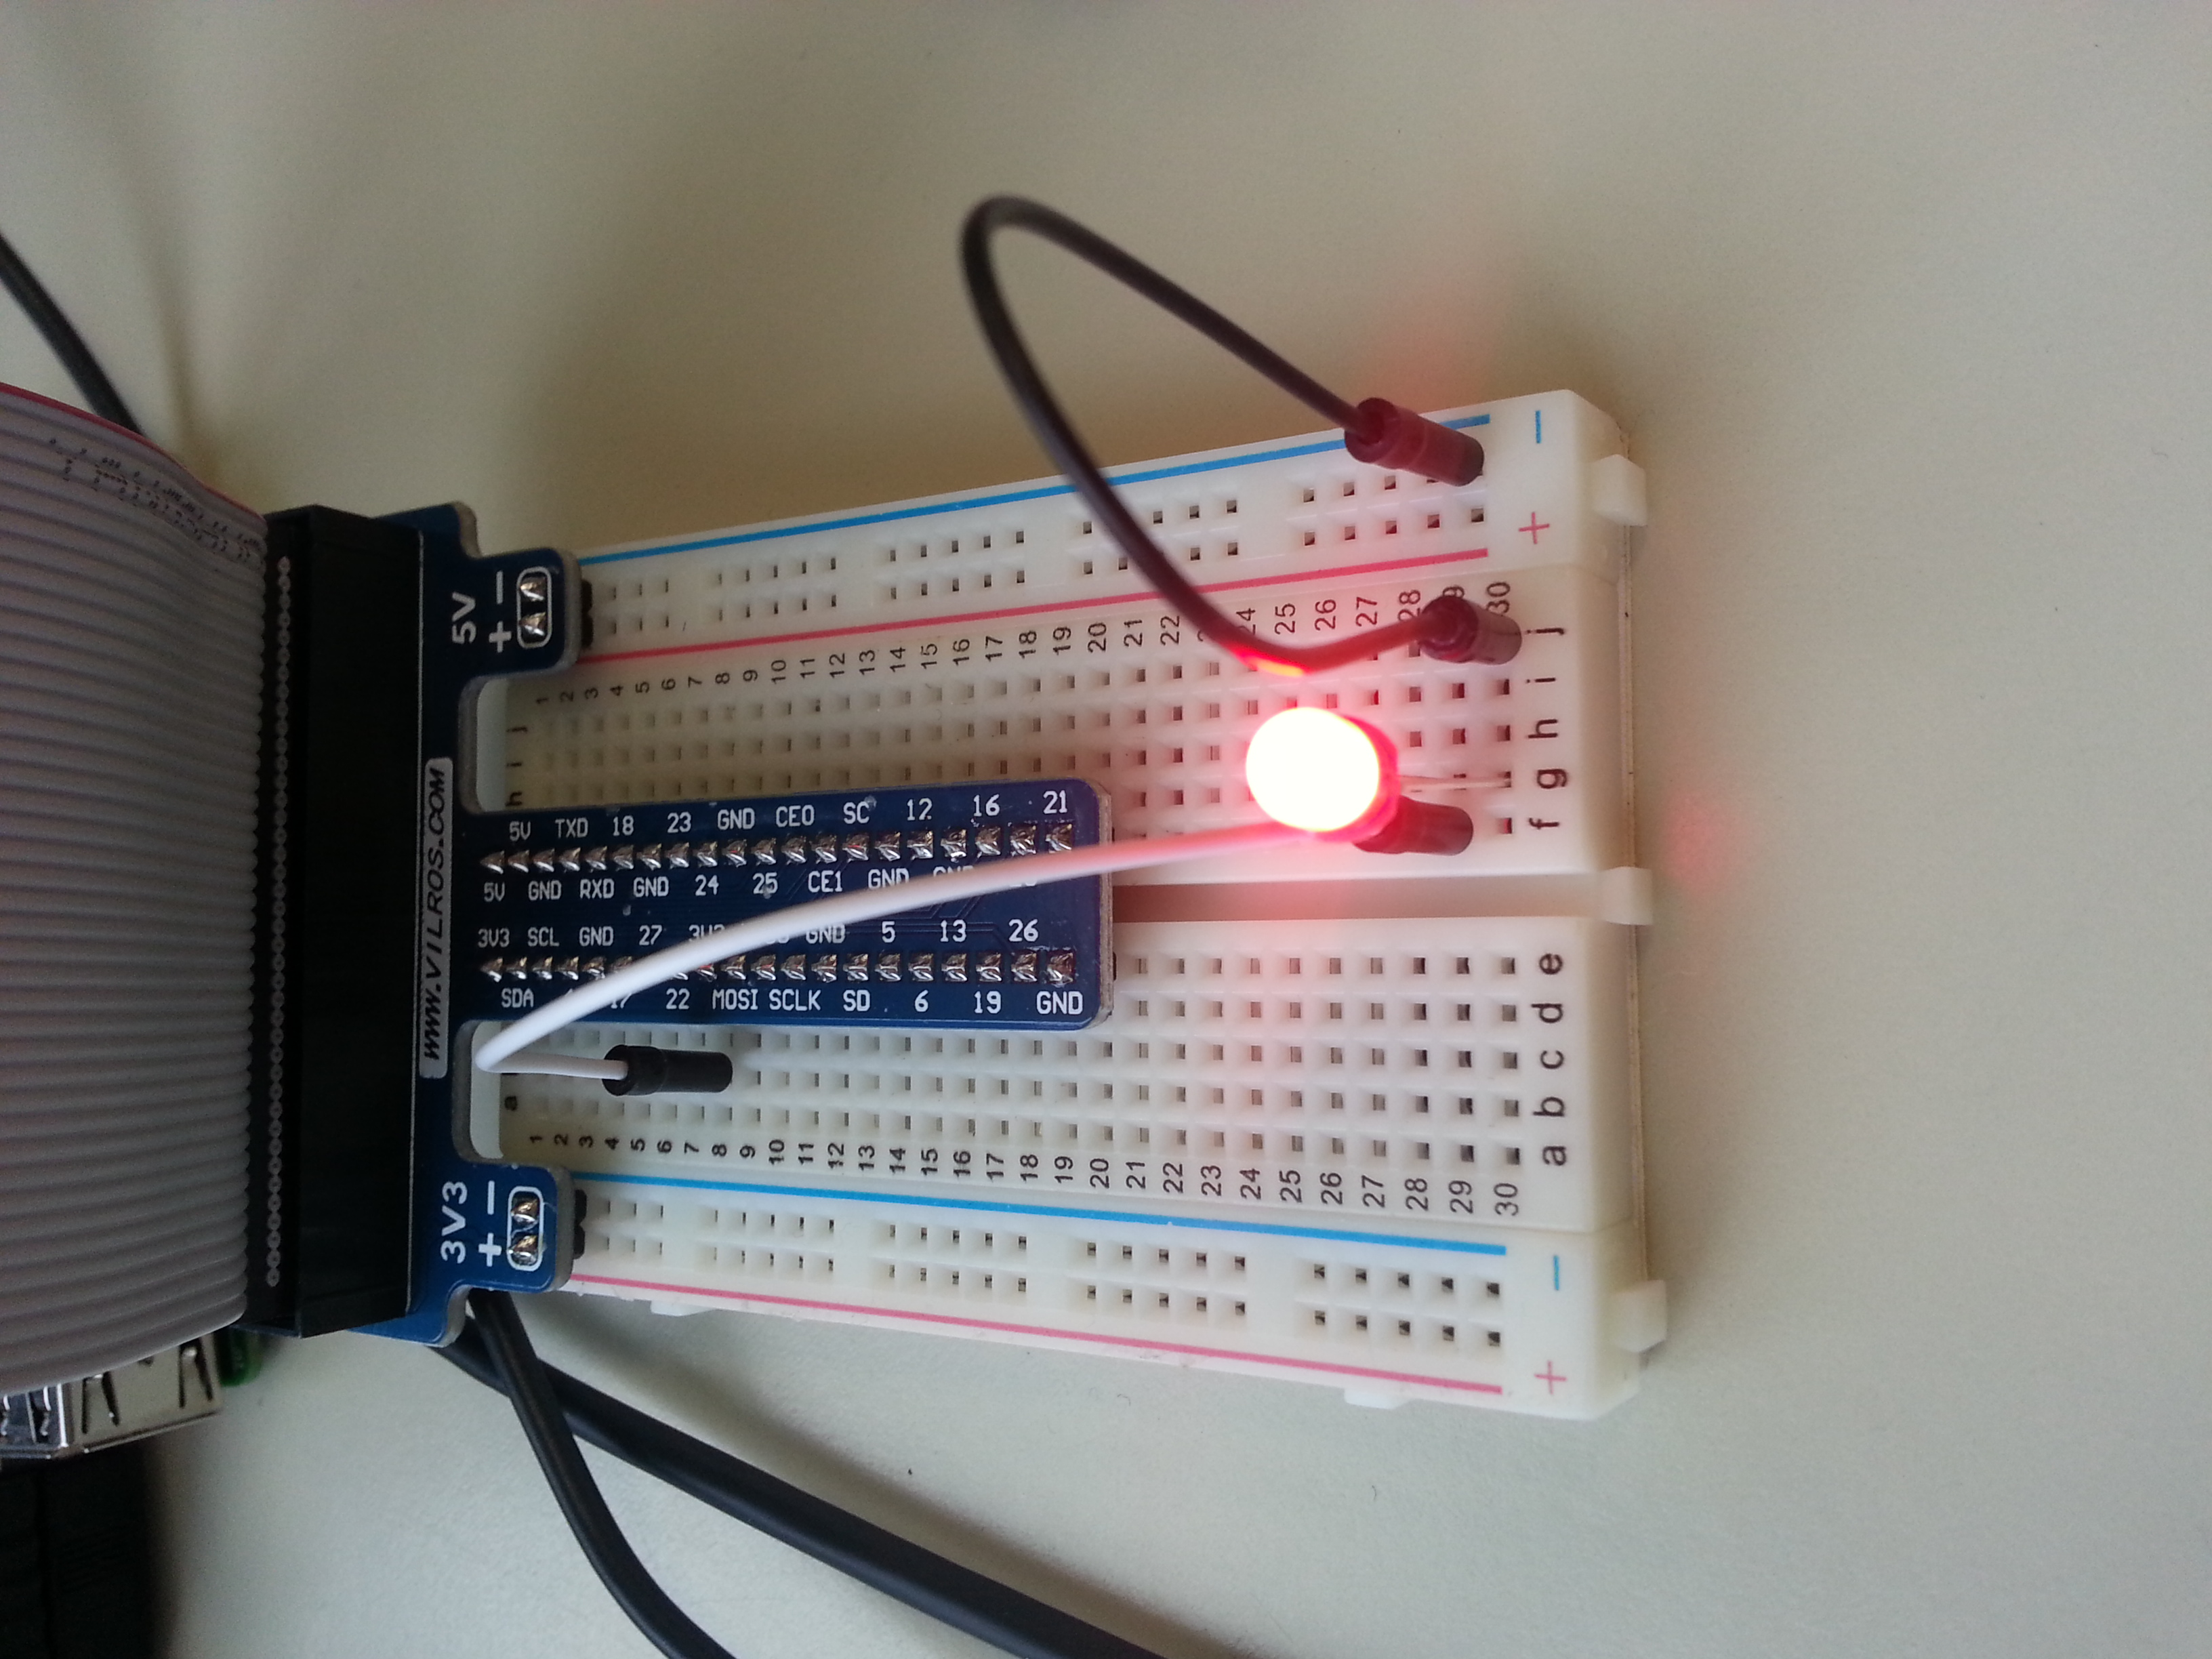
\includegraphics[width=\textwidth]{Test_unitaire/Rpi/img3.jpg}
  \caption{Allumage d'une LED par Raspberry Pi}
  \label{figure:led}
\end{figure}

\begin{figure}[!h]
  \centering
  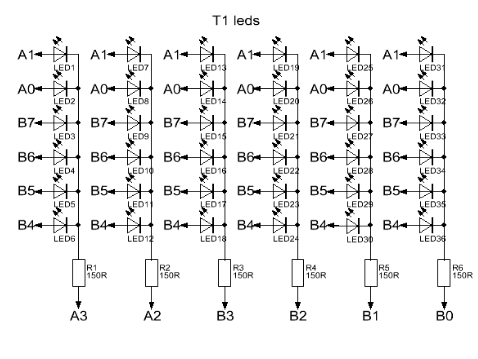
\includegraphics[width=0.8\textwidth]{Test_unitaire/Rpi/led.png}
  \caption{Méthode de connexion des leds dans le Montréal}  
  \label{figure:ledMontreal}
\end{figure}
\begin{figure}[!h]
  \centering
  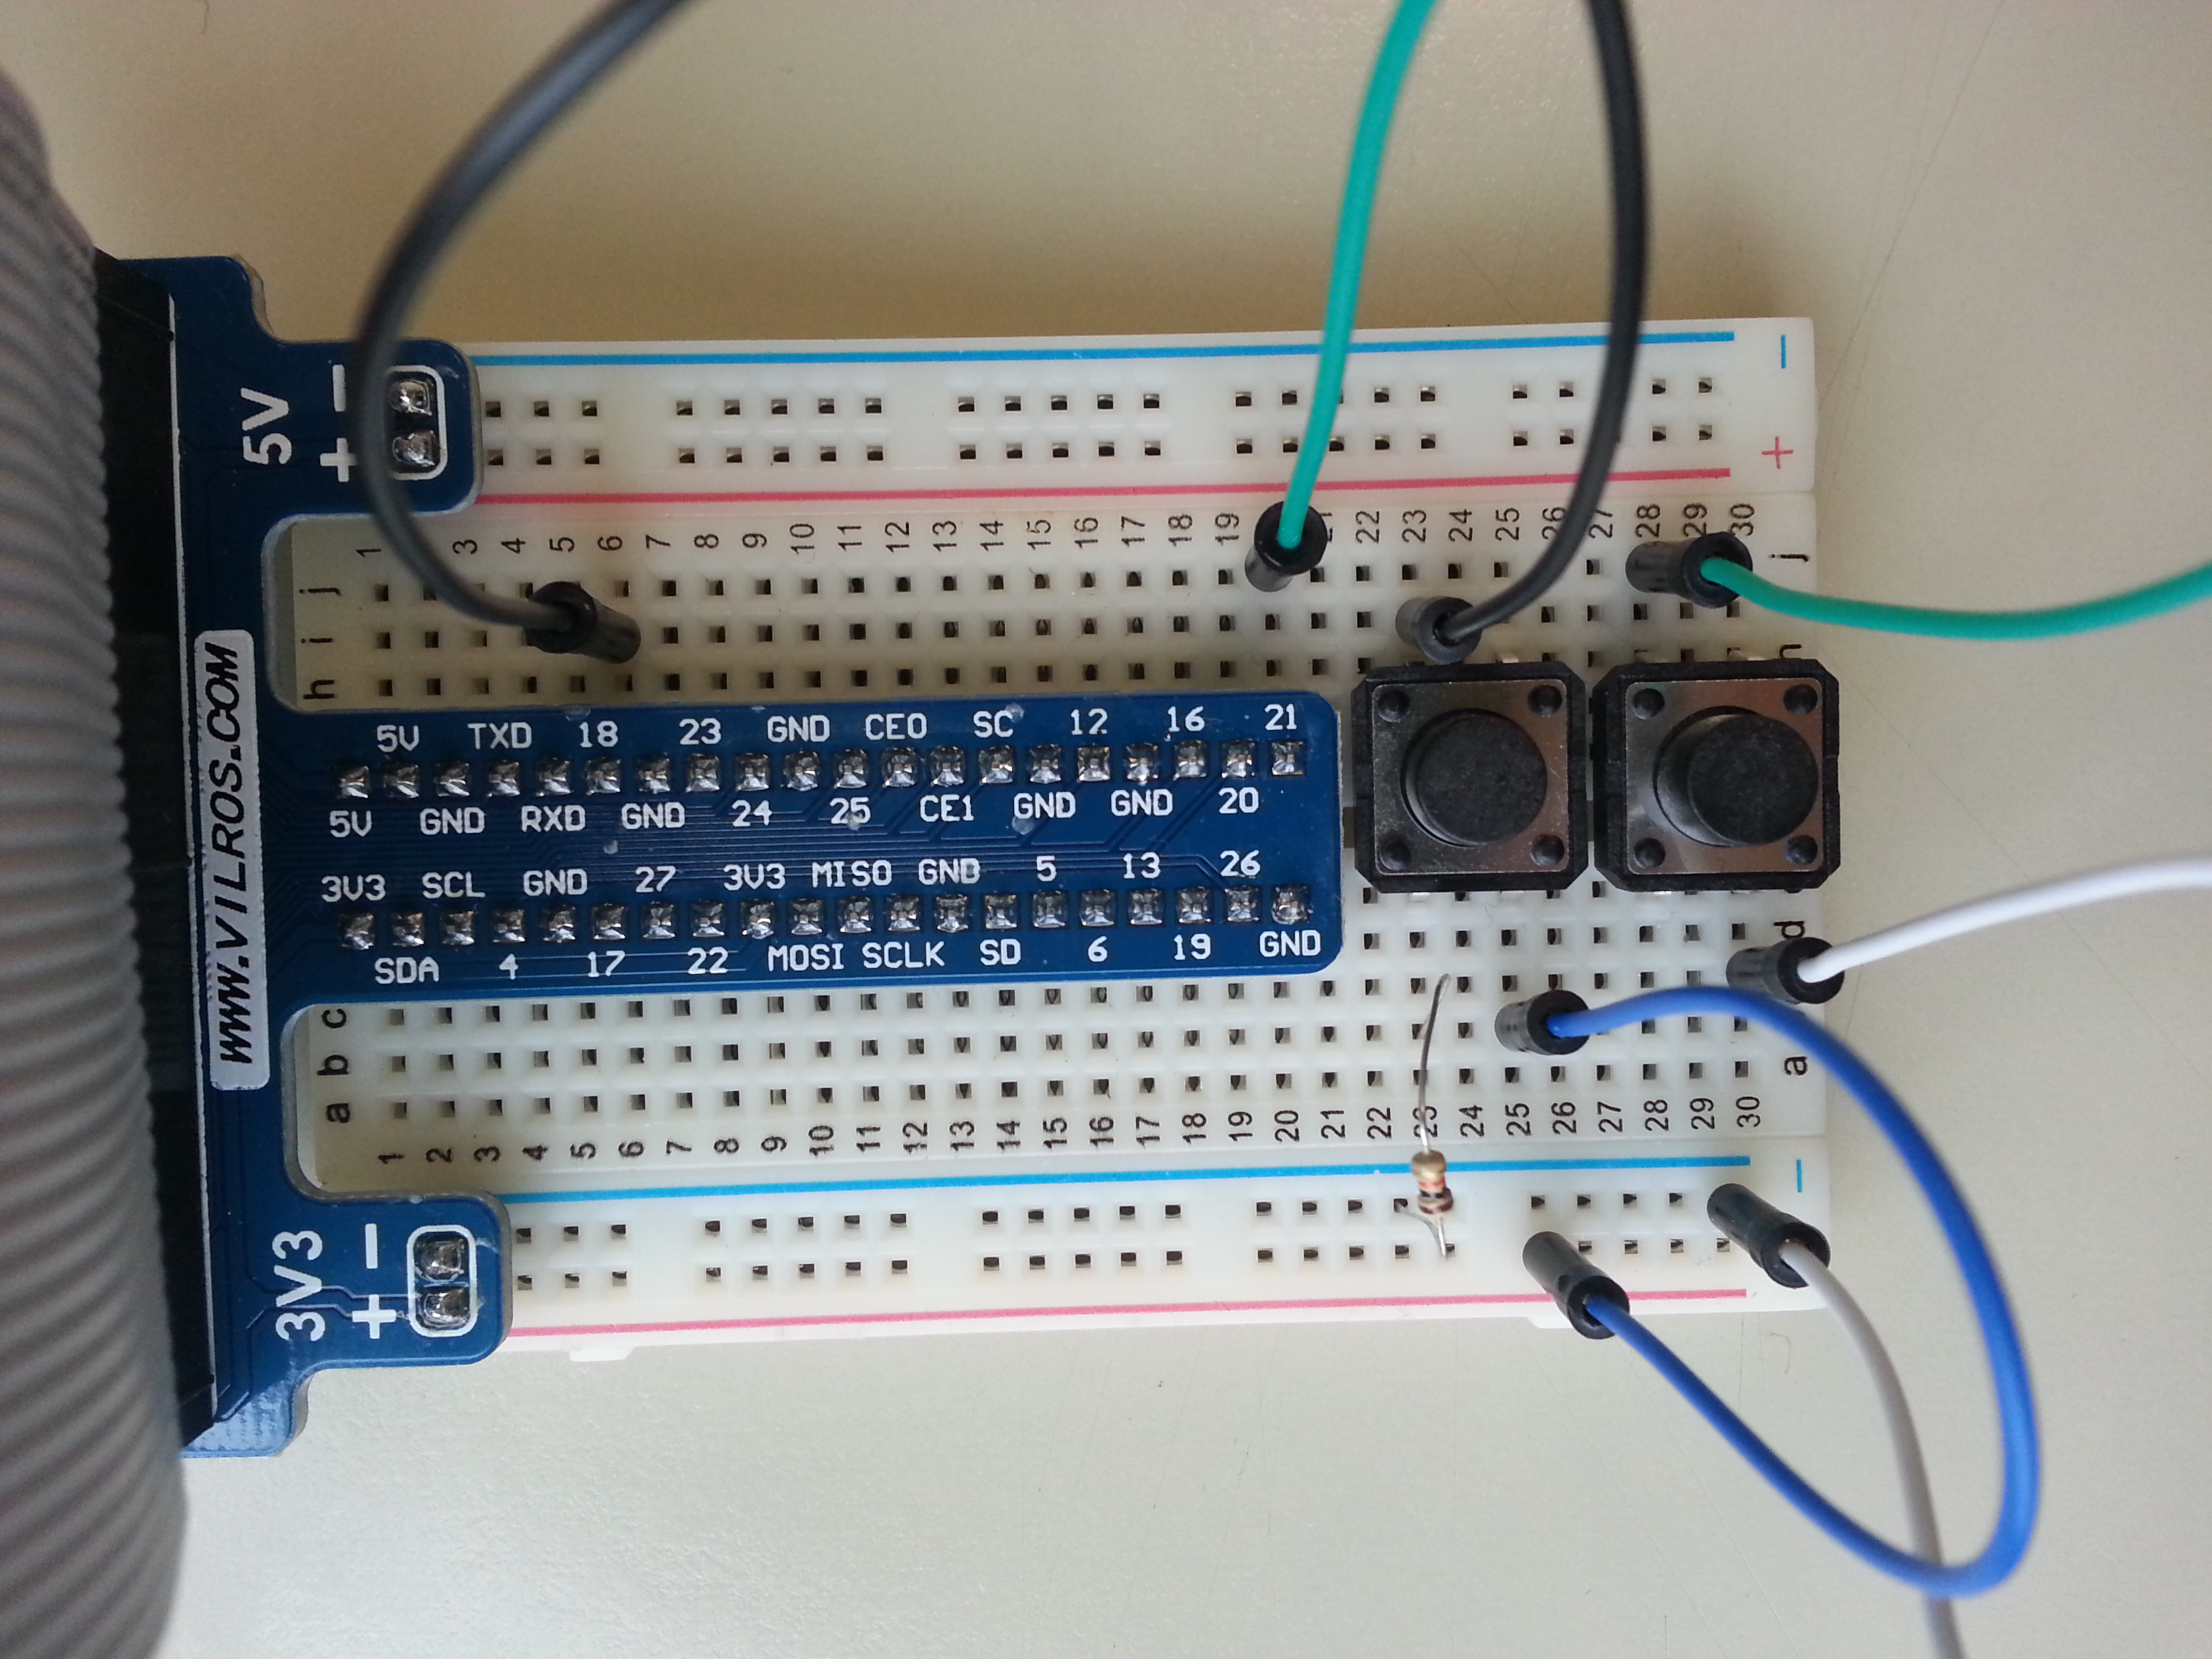
\includegraphics[width=\textwidth]{Test_unitaire/Rpi/img4.jpg}  
  \caption{Système modélisant une LED}
  \label{figure:test}
\end{figure}

La sortie du Montréal 3v2 est décrite à la figure \ref{figure:ledMontreal}. On constate que le pic qui permet l'affichage à 12 sortie qui lui permet de gérer 24 LED. Pour connaître quelle LED est allumé, il faut savoir laquelle des entré A1,A0,B7,B6,B5,B4 à un front montant et laquelle des entrées B0,B1,B2,B3,A3,A2 à un front descendant.

Pour modéliser une LED en entré du Raspberry Pi, nous avons positionné 2 boutons poussoirs (voir figure \ref{figure:test}). Le premier permets de réaliser le front montant et le second le front descendant. Ainsi en positionnant ces boutons au bon endroit par rapport au port GPIO du raspberry il est possible de connaître quelle LED on a simuler.

Nous avons réaliser un script python qui lié les entrées du raspberry avec les sortie du pic. Puis nous avons tester en simulant une LED comme décrit précédemment.

On peut constater que l'expérience est un succès car le raspberry pi nous renvoie bien le numéro de la LED que nous voulions tester.


\section{Android}

Les premiers tests de l'application Android eétaient de simples tentatives de connections avec transmission de messages simples pour vérifier le bon fonctionnement des socket Web. 
Une fois l'application terminée une série de tests plus complets ont été effectués pour simuler le comportement global de l'application en conditions réelles.
~\\
Le premier test d'intégration réalisé simule une succession de quatres instances de communication entre le client Android et le serveur. L'objectif est de simuler la transition d'un état "Rien à Signaler" vers un état "Drone détecté", et de vérifier l'exactitude des informations transmises. Pour visualiser le comportement du téléphone nous avons utilisé l'outil "logcat" du logiciel de programmation Android Studio qui permet de visualiser en temps réel les registres du téléphone. 

\begin{figure}[!h]
  \centering
  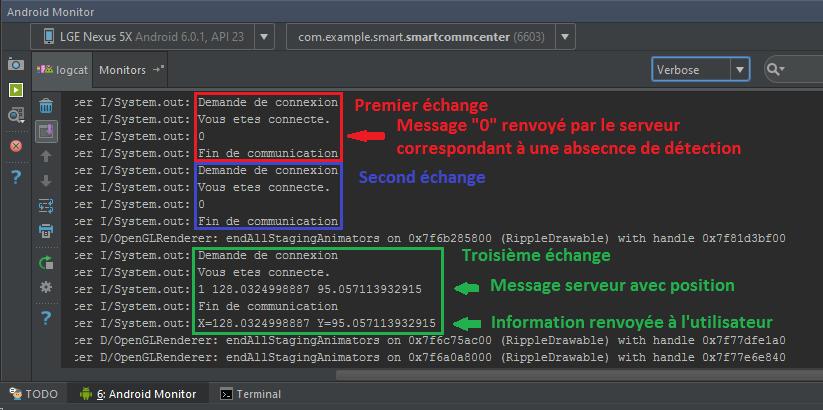
\includegraphics[width=\textwidth]{logcat}  
  \caption{Premier test : communication}
\end{figure}

Sur cette image on peut visualiser les trois premiers échanges. Les deux premières requêtes ne donne lieu à aucun changement sur l'application car aucun drone simulé n'a été détecté.
Le troisième échange résulte de l'entrée d'un drone dans la zone simulée. On d'abord peux visualiser le message brut reçu par l'application puis dans un second temps la chaine de caractères formatée par l'application avant qu'elle soit affichée par l'interface.
~\\
Le second test d'intégration lié à l'application avait pour but de vérifier le bon affichage des erreurs de connexion sur l'application Android pour éviter toute ambiguïté. 

\begin{figure}[!h]
  \centering
  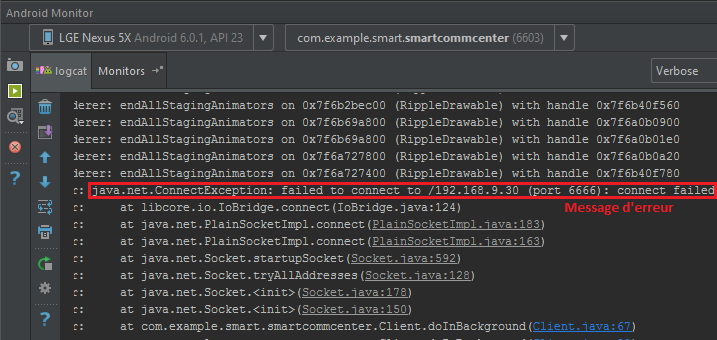
\includegraphics[width=\textwidth]{log_error}  
  \caption{Second test : erreurs}
\end{figure}

\newpage %% a virer si ça gène

\begin{wrapfigure}{r}{0.5\textwidth}

  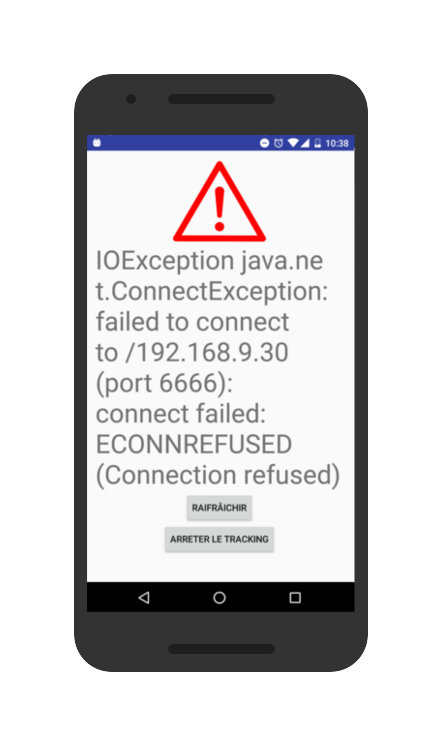
\includegraphics[width=0.25\textwidth]{error_co}
  \caption{Message d'erreur sur l'application}
\end{wrapfigure}

En cas d'erreur le message est bien visible dans les logs et L'application ne s'est pas bloquée. Celle-ci sera donc capable de bien différencier une absence de détection d'une erreur de connections tout en restant prête à renvoyer une requête au serveur. De plus, le message d'erreur est bien affiché dans son intégralité sur l'interface de l'application. elle est ici réglée en mode "Debug" pour afficher un maximum d'informations.



%%% Local Variables: 
%%% mode: latex
%%% TeX-master: "../rapport"
%%% End: 